% Appendix B

\chapter{Results for 4X scale} % Main appendix title

\label{AppendixB} % For referencing this appendix elsewhere, use \ref{AppendixB}

    \begin{figure*}
        \centering
        \begin{subfigure}[b]{0.75\textwidth}
            \centering
            \includegraphics[width=\textwidth]{Figures/2X/Cyberpunk/be15968553390b112e723e8773910e11.png}
            \caption{High Resolution}
        \end{subfigure}
        \vskip\baselineskip
        \begin{subfigure}[b]{0.475\textwidth}
            \centering
            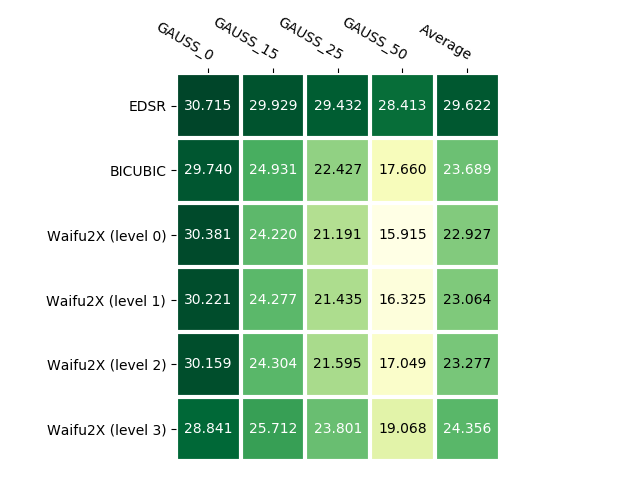
\includegraphics[width=\textwidth]{Figures/4X/Cyberpunk/PSNR_GAUSS.png}
            \caption{PSNR results with gaussian noise}
        \end{subfigure}
        \hfill
        \begin{subfigure}[b]{0.475\textwidth}  
            \centering 
            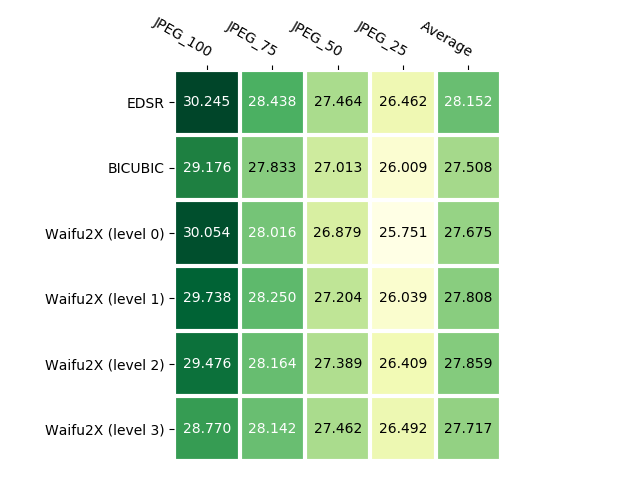
\includegraphics[width=\textwidth]{Figures/4X/Cyberpunk/PSNR_JPEG.png}
            \caption{PSNR results with JPEG noise}
        \end{subfigure}
        \vskip\baselineskip
        \begin{subfigure}[b]{0.475\textwidth}   
            \centering 
            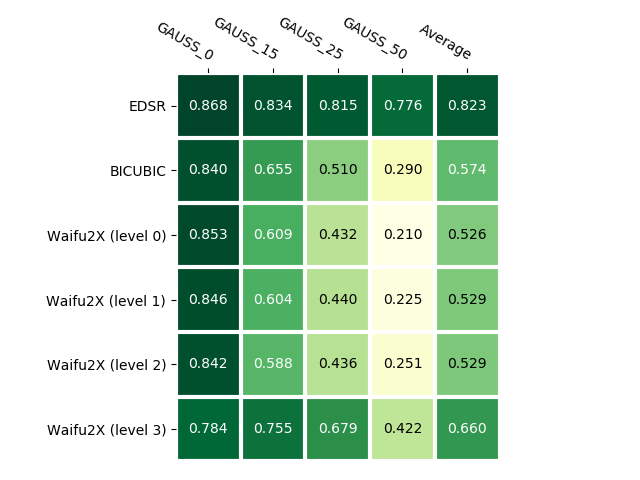
\includegraphics[width=\textwidth]{Figures/4X/Cyberpunk/SSIM_GAUSS.png}
            \caption{SSIM results with gaussian noise}
        \end{subfigure}
        \quad
        \begin{subfigure}[b]{0.475\textwidth}   
            \centering 
            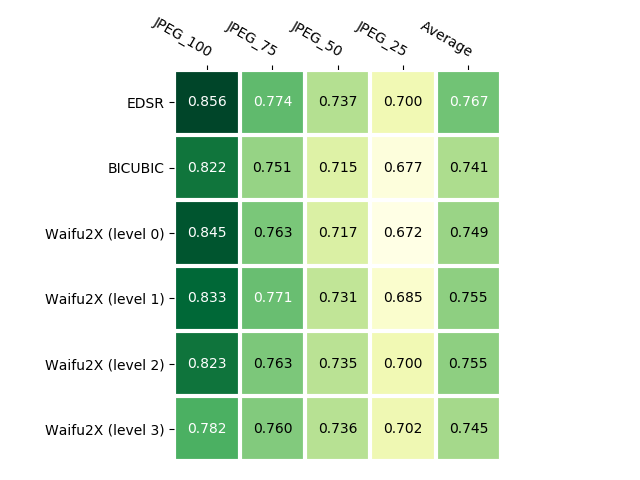
\includegraphics[width=\textwidth]{Figures/4X/Cyberpunk/SSIM_JPEG.png}
            \caption{SSIM results with JPEG noise}
        \end{subfigure}
        \caption{PSNR and SSIM results on the shown image}
    \end{figure*}
    
    \begin{figure*}
        \centering
        \begin{subfigure}[b]{0.75\textwidth}
            \centering
            \includegraphics[width=\textwidth]{Figures/2X/Tiger/image.png}
            \caption{High Resolution}
        \end{subfigure}
        \vskip\baselineskip
        \begin{subfigure}[b]{0.475\textwidth}
            \centering
            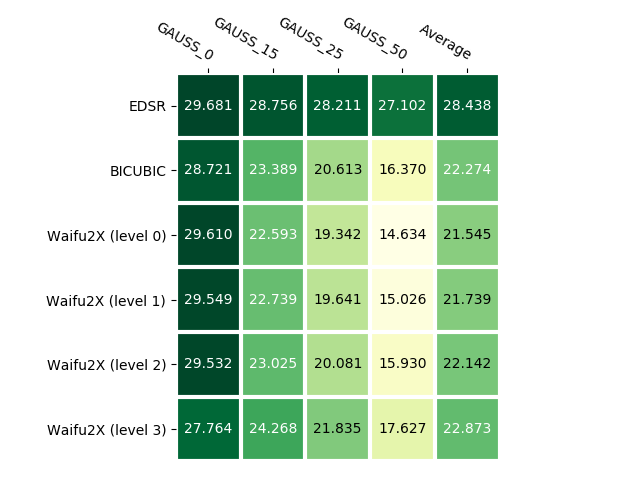
\includegraphics[width=\textwidth]{Figures/4X/Tiger/PSNR_GAUSS.png}
            \caption{PSNR results with gaussian noise}
        \end{subfigure}
        \hfill
        \begin{subfigure}[b]{0.475\textwidth}  
            \centering 
            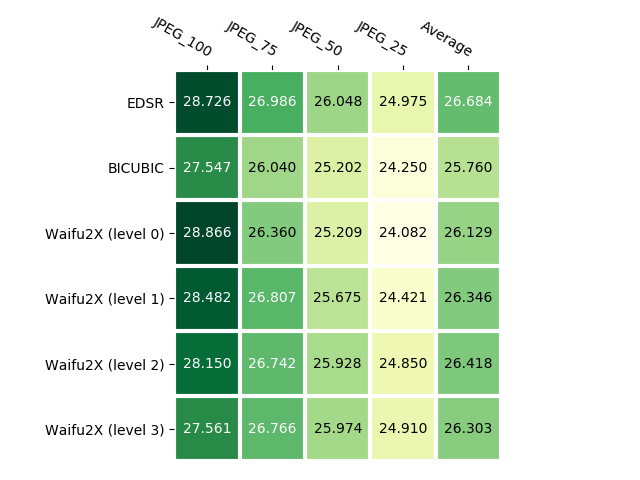
\includegraphics[width=\textwidth]{Figures/4X/Tiger/PSNR_JPEG.png}
            \caption{PSNR results with JPEG noise}
        \end{subfigure}
        \vskip\baselineskip
        \begin{subfigure}[b]{0.475\textwidth}   
            \centering 
            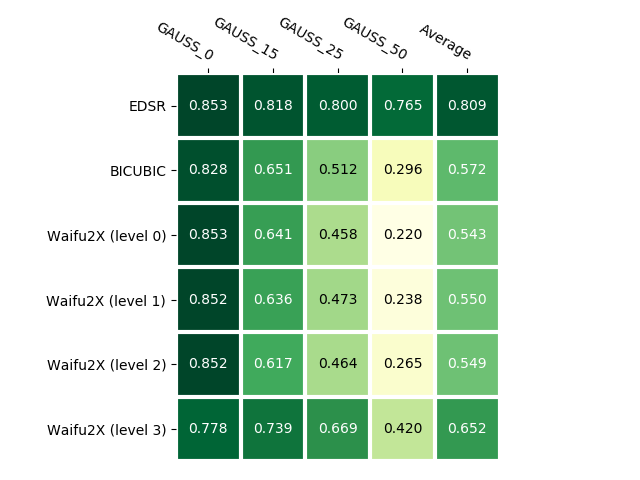
\includegraphics[width=\textwidth]{Figures/4X/Tiger/SSIM_GAUSS.png}
            \caption{SSIM results with gaussian noise}
        \end{subfigure}
        \quad
        \begin{subfigure}[b]{0.475\textwidth}   
            \centering 
            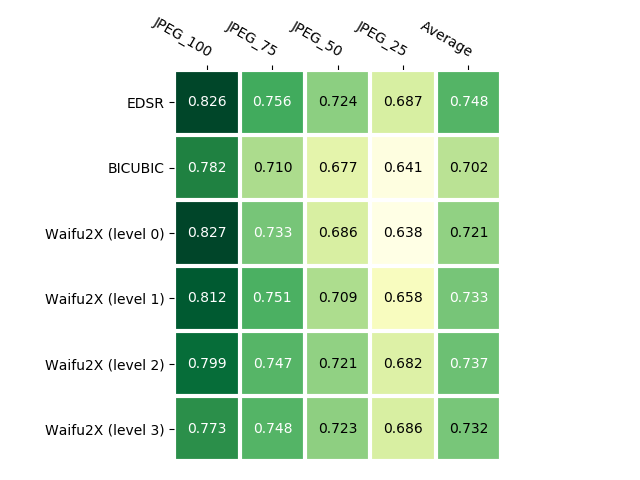
\includegraphics[width=\textwidth]{Figures/4X/Tiger/SSIM_JPEG.png}
            \caption{SSIM results with JPEG noise}
        \end{subfigure}
        \caption{PSNR and SSIM results on the shown image}
    \end{figure*}
    
        \begin{figure*}
        \centering
        \begin{subfigure}[b]{0.75\textwidth}
            \centering
            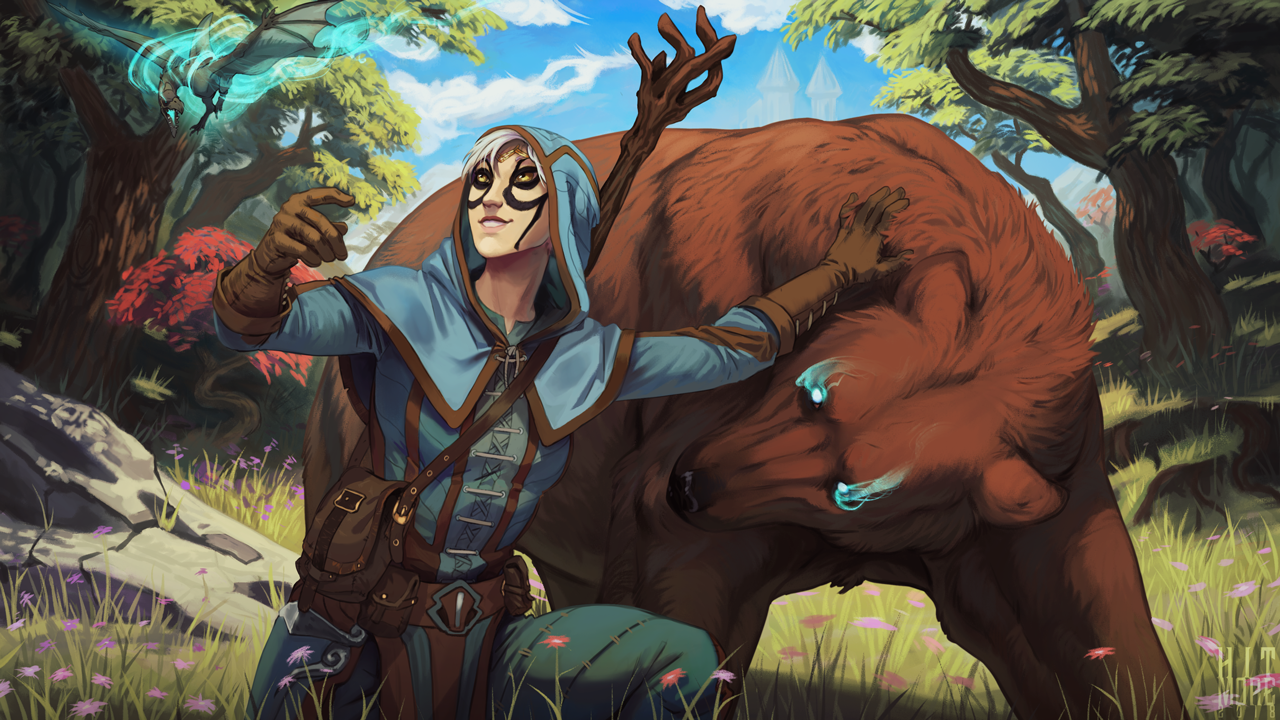
\includegraphics[width=\textwidth]{Figures/2X/Bear/image.png}
            \caption{High Resolution}
        \end{subfigure}
        \vskip\baselineskip
        \begin{subfigure}[b]{0.475\textwidth}
            \centering
            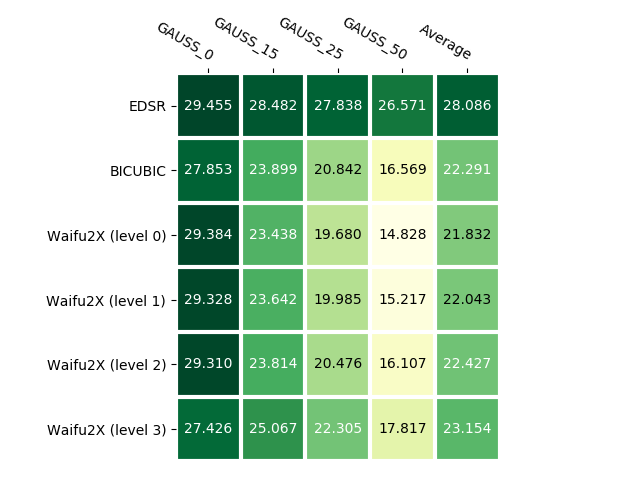
\includegraphics[width=\textwidth]{Figures/4X/Bear/PSNR_GAUSS.png}
            \caption{PSNR results with gaussian noise}
        \end{subfigure}
        \hfill
        \begin{subfigure}[b]{0.475\textwidth}  
            \centering 
            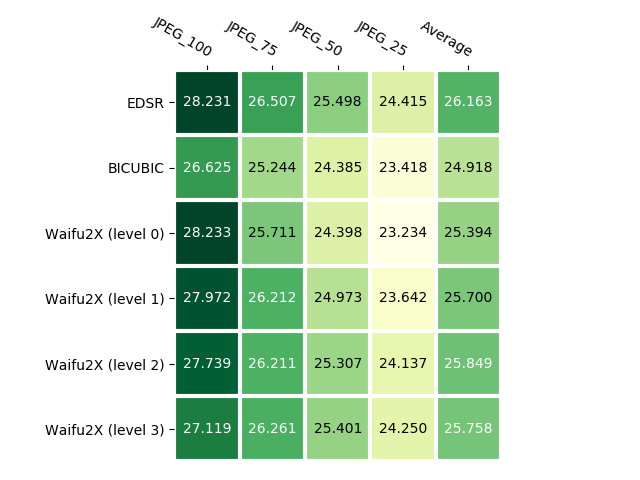
\includegraphics[width=\textwidth]{Figures/4X/Bear/PSNR_JPEG.png}
            \caption{PSNR results with JPEG noise}
        \end{subfigure}
        \vskip\baselineskip
        \begin{subfigure}[b]{0.475\textwidth}   
            \centering 
            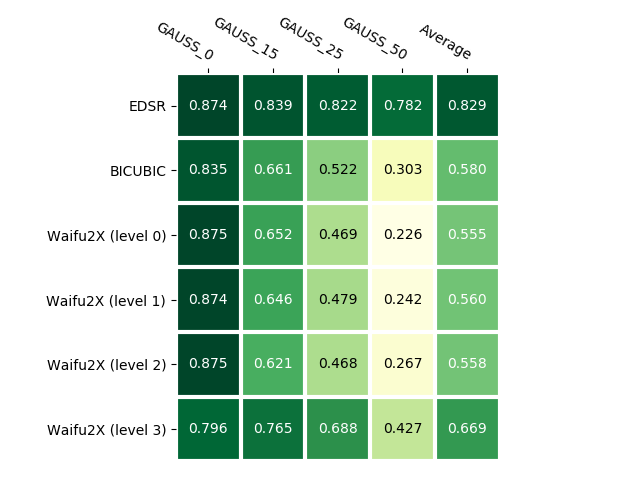
\includegraphics[width=\textwidth]{Figures/4X/Bear/SSIM_GAUSS.png}
            \caption{SSIM results with gaussian noise}
        \end{subfigure}
        \quad
        \begin{subfigure}[b]{0.475\textwidth}   
            \centering 
            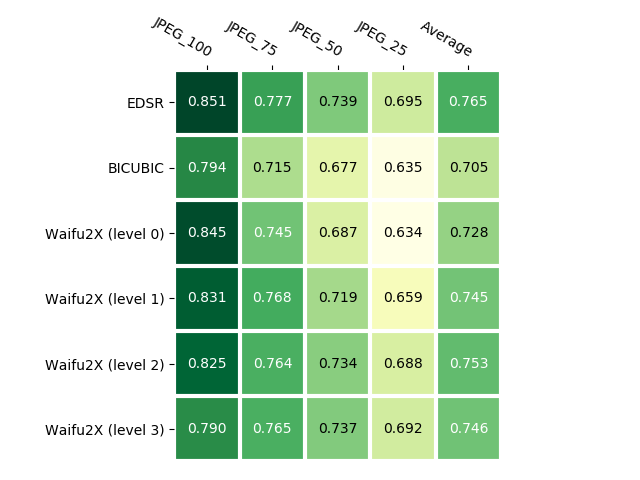
\includegraphics[width=\textwidth]{Figures/4X/Bear/SSIM_JPEG.png}
            \caption{SSIM results with JPEG noise}
        \end{subfigure}
        \caption{PSNR and SSIM results on the shown image}
    \end{figure*}
    
        \begin{figure*}
        \centering
        \begin{subfigure}[b]{0.75\textwidth}
            \centering
            \includegraphics[width=\textwidth]{Figures/2X/Catch/image.png}
            \caption{High Resolution}
        \end{subfigure}
        \vskip\baselineskip
        \begin{subfigure}[b]{0.475\textwidth}
            \centering
            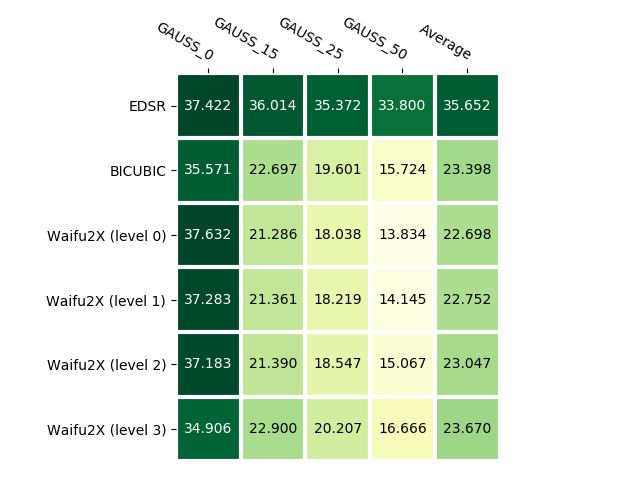
\includegraphics[width=\textwidth]{Figures/4X/Catch/PSNR_GAUSS.png}
            \caption{PSNR results with gaussian noise}
        \end{subfigure}
        \hfill
        \begin{subfigure}[b]{0.475\textwidth}  
            \centering 
            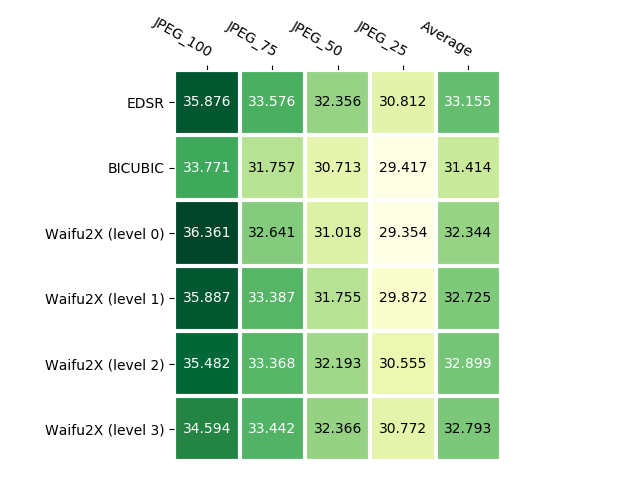
\includegraphics[width=\textwidth]{Figures/4X/Catch/PSNR_JPEG.png}
            \caption{PSNR results with JPEG noise}
        \end{subfigure}
        \vskip\baselineskip
        \begin{subfigure}[b]{0.475\textwidth}   
            \centering 
            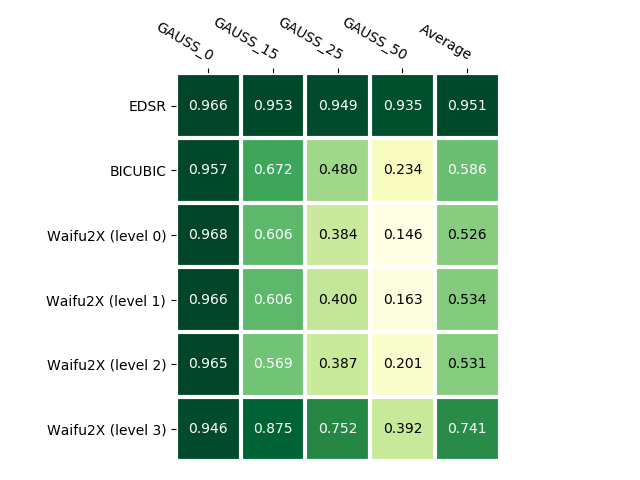
\includegraphics[width=\textwidth]{Figures/4X/Catch/SSIM_GAUSS.png}
            \caption{SSIM results with gaussian noise}
        \end{subfigure}
        \quad
        \begin{subfigure}[b]{0.475\textwidth}   
            \centering 
            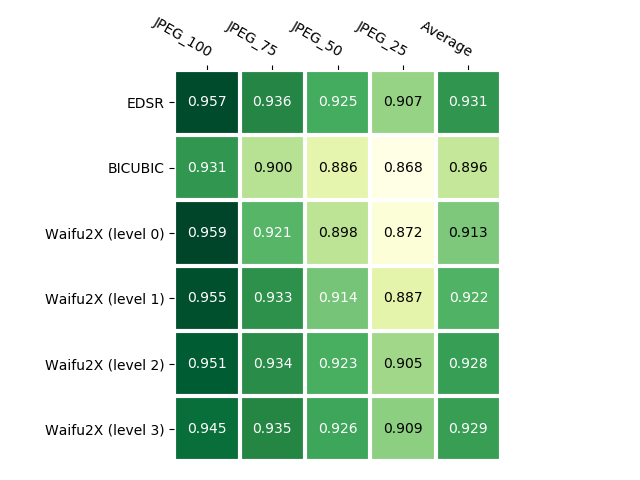
\includegraphics[width=\textwidth]{Figures/4X/Catch/SSIM_JPEG.png}
            \caption{SSIM results with JPEG noise}
        \end{subfigure}
        \caption{PSNR and SSIM results on the shown image}
    \end{figure*}
    
            \begin{figure*}
        \centering
        \begin{subfigure}[b]{0.75\textwidth}
            \centering
            \includegraphics[width=\textwidth]{Figures/2X/Coffee/image.png}
            \caption{High Resolution}
        \end{subfigure}
        \vskip\baselineskip
        \begin{subfigure}[b]{0.475\textwidth}
            \centering
            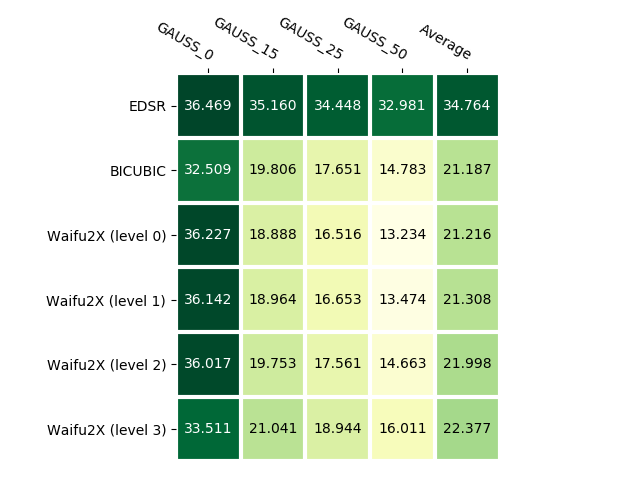
\includegraphics[width=\textwidth]{Figures/4X/Coffee/PSNR_GAUSS.png}
            \caption{PSNR results with gaussian noise}
        \end{subfigure}
        \hfill
        \begin{subfigure}[b]{0.475\textwidth}  
            \centering 
            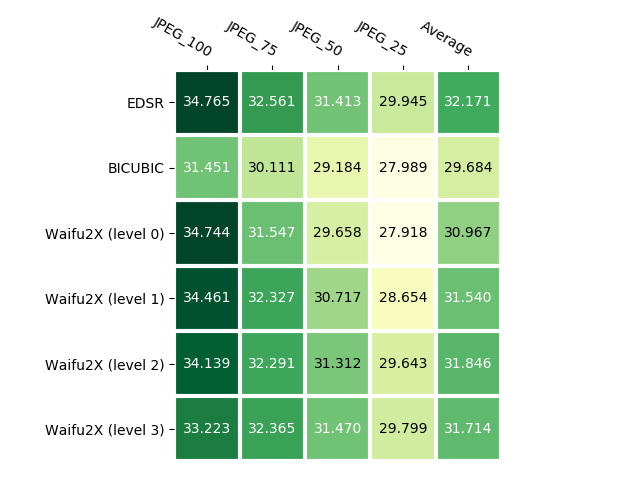
\includegraphics[width=\textwidth]{Figures/4X/Coffee/PSNR_JPEG.png}
            \caption{PSNR results with JPEG noise}
        \end{subfigure}
        \vskip\baselineskip
        \begin{subfigure}[b]{0.475\textwidth}   
            \centering 
            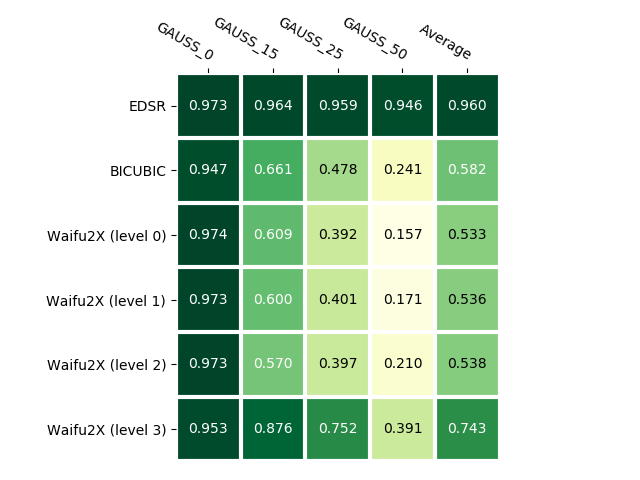
\includegraphics[width=\textwidth]{Figures/4X/Coffee/SSIM_GAUSS.png}
            \caption{SSIM results with gaussian noise}
        \end{subfigure}
        \quad
        \begin{subfigure}[b]{0.475\textwidth}   
            \centering 
            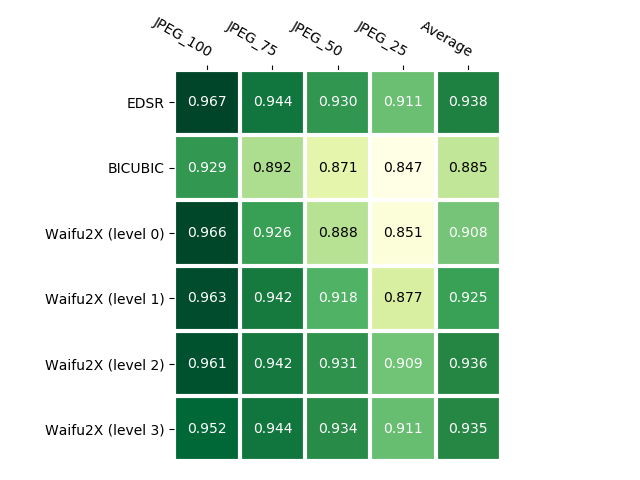
\includegraphics[width=\textwidth]{Figures/4X/Coffee/SSIM_JPEG.png}
            \caption{SSIM results with JPEG noise}
        \end{subfigure}
        \caption{PSNR and SSIM results on the shown image}
    \end{figure*}
    
            \begin{figure*}
        \centering
        \begin{subfigure}[b]{0.75\textwidth}
            \centering
            
\includegraphics[width=\textwidth]{Figures/2X/Crow/image.png}
            \caption{High Resolution}
        \end{subfigure}
        \vskip\baselineskip
        \begin{subfigure}[b]{0.475\textwidth}
            \centering
            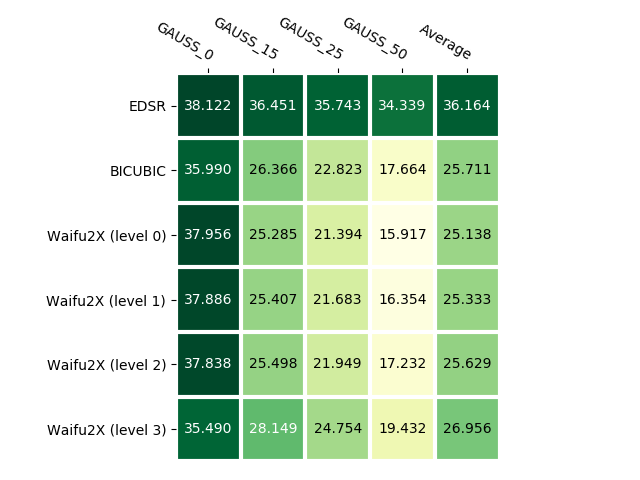
\includegraphics[width=\textwidth]{Figures/4X/Crow/PSNR_GAUSS.png}
            \caption{PSNR results with gaussian noise}
        \end{subfigure}
        \hfill
        \begin{subfigure}[b]{0.475\textwidth}  
            \centering 
            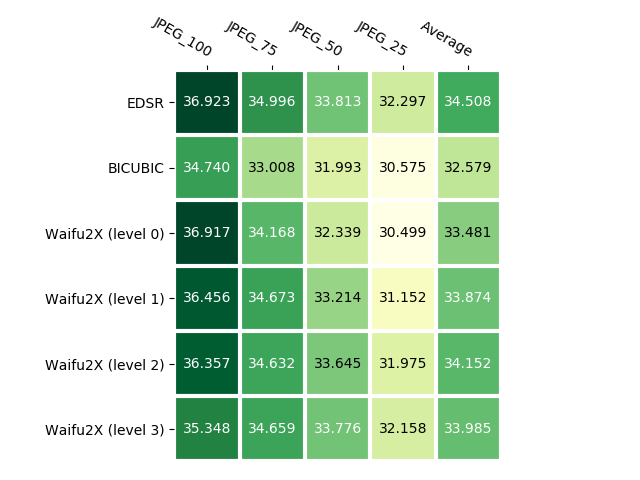
\includegraphics[width=\textwidth]{Figures/4X/Crow/PSNR_JPEG.png}
            \caption{PSNR results with JPEG noise}
        \end{subfigure}
        \vskip\baselineskip
        \begin{subfigure}[b]{0.475\textwidth}   
            \centering 
            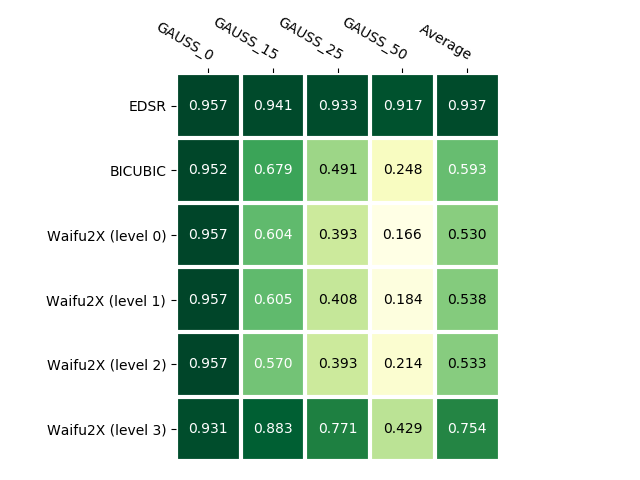
\includegraphics[width=\textwidth]{Figures/4X/Crow/SSIM_GAUSS.png}
            \caption{SSIM results with gaussian noise}
        \end{subfigure}
        \quad
        \begin{subfigure}[b]{0.475\textwidth}   
            \centering 
            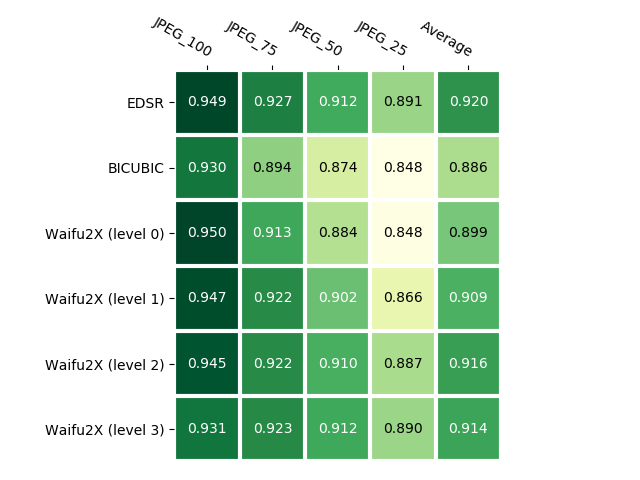
\includegraphics[width=\textwidth]{Figures/4X/Crow/SSIM_JPEG.png}
            \caption{SSIM results with JPEG noise}
        \end{subfigure}
        \caption{PSNR and SSIM results on the shown image}
    \end{figure*}
    
            \begin{figure*}
        \centering
        \begin{subfigure}[b]{0.75\textwidth}
            \centering
            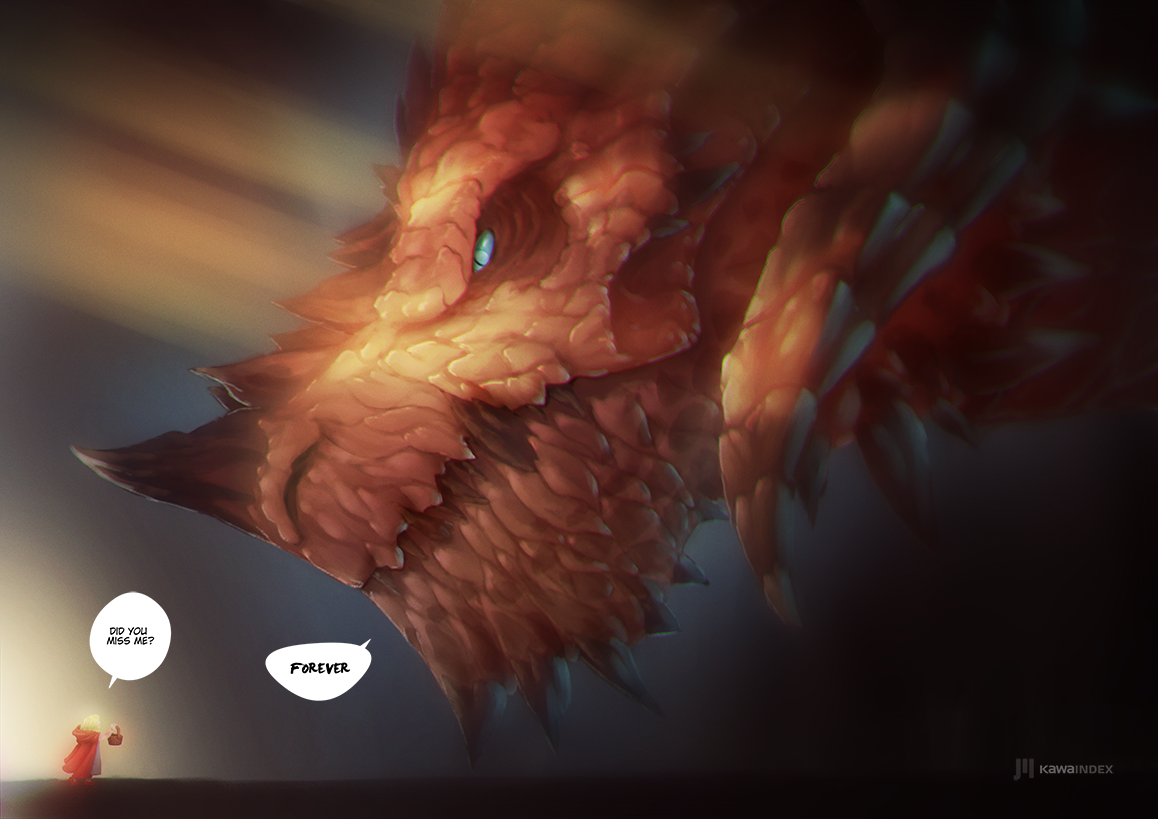
\includegraphics[width=\textwidth]{Figures/2X/Dragon/image.png}
            \caption{High Resolution}
        \end{subfigure}
        \vskip\baselineskip
        \begin{subfigure}[b]{0.475\textwidth}
            \centering
            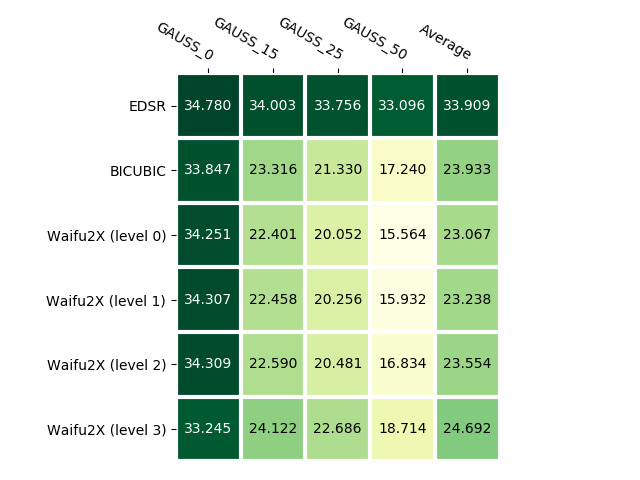
\includegraphics[width=\textwidth]{Figures/4X/Dragon/PSNR_GAUSS.png}
            \caption{PSNR results with gaussian noise}
        \end{subfigure}
        \hfill
        \begin{subfigure}[b]{0.475\textwidth}  
            \centering 
            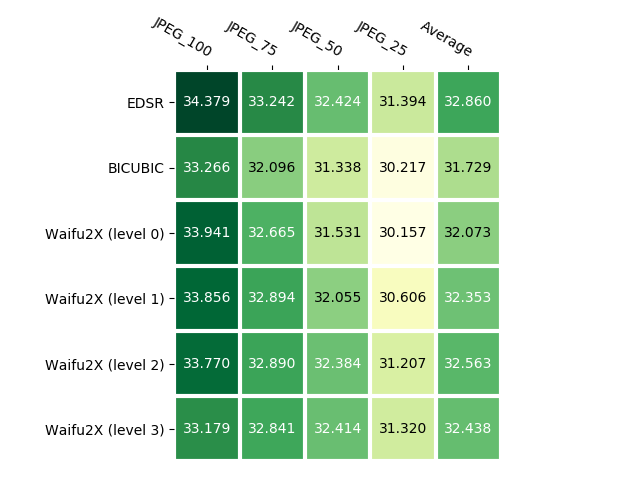
\includegraphics[width=\textwidth]{Figures/4X/Dragon/PSNR_JPEG.png}
            \caption{PSNR results with JPEG noise}
        \end{subfigure}
        \vskip\baselineskip
        \begin{subfigure}[b]{0.475\textwidth}   
            \centering 
            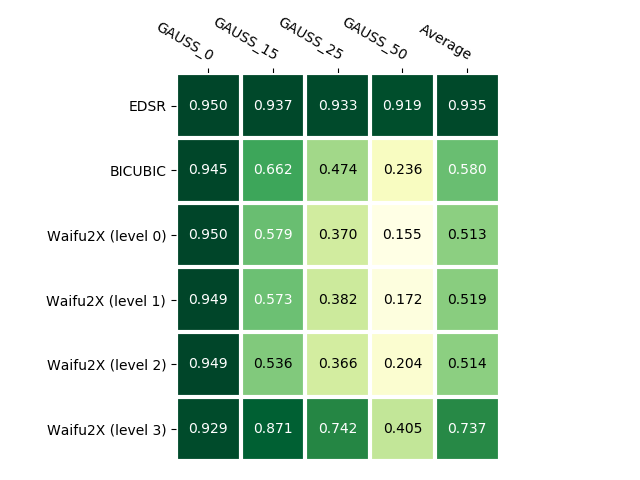
\includegraphics[width=\textwidth]{Figures/4X/Dragon/SSIM_GAUSS.png}
            \caption{SSIM results with gaussian noise}
        \end{subfigure}
        \quad
        \begin{subfigure}[b]{0.475\textwidth}   
            \centering 
            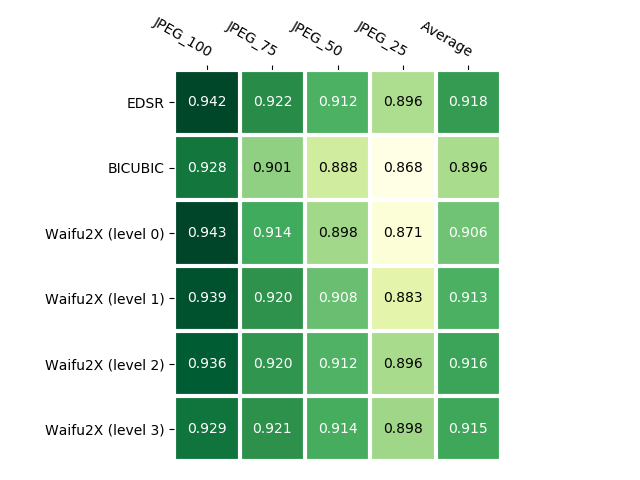
\includegraphics[width=\textwidth]{Figures/4X/Dragon/SSIM_JPEG.png}
            \caption{SSIM results with JPEG noise}
        \end{subfigure}
        \caption{PSNR and SSIM results on the shown image}
    \end{figure*}